\documentclass[12pt]{article}

\usepackage[T1]{fontenc}
\usepackage[utf8]{inputenc}
\usepackage{lmodern}

\usepackage[ngerman, english]{babel}

\usepackage[ngerman]{translator}

\usepackage{csquotes}

\usepackage{amsmath}

\usepackage[separate-uncertainty=true]{siunitx}

\usepackage{xcolor}

\usepackage{geometry}
\geometry{a4paper, top=15mm, left=20mm, right=20mm, bottom=30mm, headsep=10mm, footskip=20mm}

\usepackage[backend=biber, style=numeric]{biblatex}
\addbibresource{bib/references.bib}

\usepackage{graphicx}

\setlength{\columnsep}{10mm} % set length of the gap between two columns
\setlength{\parindent}{0mm} % set length of indentation of a paragraph
\setlength{\parskip}{2mm} % set length of the gap between two paragraphs
\setlength{\emergencystretch}{\hsize} % allow big stretch to avoid overful \hbox without using \sloppy

\linespread{1.1} % set gap between lines

\usepackage{adjustbox} % used for \adjustbox

\usepackage{units} % used for \nicefrac

\usepackage{hyperref} % automatically create clickable links

\usepackage{multicol} % used for \begin{multicols} to create a column layout

\usepackage{caption} % used for \captionsetup and \captionof

\usepackage{titlesec} % used to format section, subsection and subsubsection
\titleformat*{\section}{\normalfont\sffamily\Large\bfseries}
\titleformat*{\subsection}{\normalfont\sffamily\large\bfseries}
\titleformat*{\subsubsection}{\normalfont\sffamily\normalsize\bfseries}
\titlespacing{\section}{0pt}{*3}{*1}
\titlespacing{\subsection}{0pt}{*3}{*1}
\titlespacing{\subsubsection}{0pt}{*3}{*1}

\usepackage{framed} % used for \begin{snugshade*}
\definecolor{shadecolor}{RGB}{230, 230, 230} % set background color for \begin{snugshade*}

\usepackage{booktabs} % used for \toprule, \midrule and \bottomrule with tables

\usepackage[colorinlistoftodos, prependcaption, textsize=tiny]{todonotes}

\usepackage{listings}
\lstset{
    language=Python,
    aboveskip=5mm,
    belowskip=5mm,
    numbers=left,
    stepnumber=1,
    showstringspaces=false,
    breaklines=true,
    frame=none,
    tabsize=4,
    basicstyle=\ttfamily,
    commentstyle=\color[rgb]{0.10,0.50,0.00}\ttfamily,
    keywordstyle=\color[rgb]{0.00,0.13,0.98}\ttfamily\bfseries,
    identifierstyle=,
    numberstyle=\ttfamily,
    stringstyle=\color[rgb]{0.50,0.50,0.50}\ttfamily,
    backgroundcolor=,
}
\lstset{literate=%
    {Ä}{{\"A}}1
    {Ö}{{\"O}}1
    {Ü}{{\"U}}1
    {ä}{{\"a}}1
    {ö}{{\"o}}1
    {ü}{{\"u}}1
    {ß}{{\ss}}1
}

\makeatletter
\newcommand*{\header}[1]{\gdef\@header{#1}}
\def\@maketitle{
    \begin{flushleft}
    \Large
    \textsf{\@header}
    \par
    \vskip 0mm
    \LARGE
    \textsf{\textbf{\@title}}
    \par
    \vskip 2mm
    \large
    \textsf{{\@author} | durchgeführt in der Woche vom \@date}
    \end{flushleft}
    \vskip 2mm
    }
\makeatother
 % import custom \maketitle command
\header{Lange besondere Ausarbeitung Fortgeschrittenen-Praktikum}
\title{F78 Computeransteuerung und Datenverarbeitung}
\author{Vorname Name, Vorname Name}
\date{01.01.1970}

\begin{document}

%\selectlanguage{english}
%\sisetup{locale=US}
\selectlanguage{ngerman}
\sisetup{locale=DE}

\maketitle

\begin{snugshade*}
    \section*{Abstract}
%
This article is about the experiment on coincidence spectroscopy as part of the "Fortgeschrittenenpraktukum". 
Is is meant to give a practical introduction into the methods of scintillation detectors.
The theoretical processes of radioactive decay and the interaction of the resulting $\gamma$ rays with matter are tested experimentally.
The coincidence method is used to detect the correlation of photons emitted in certain decays.

\end{snugshade*}
\section{Einleitung}

\subsection{Motivation}

Bei diesem Versuch geht es darum, Methoden der computergesteuerten Datenaufnahme und -verarbeitung kennenzulernen.
Dazu wird die Biegeschwingung eines Metallstäbchens mithilfe elektronischer Verfahren gesteuert und vermessen.
Solche mechanischen Oszillationen werden oft zur Untersuchung der elastischen Eigenschaften von Festkörpern verwendet.
Die näheren physikalischen Eigenschaften und Ergebnisse spielen in diesem Versuch nur eine untergeordnete Rolle.
Es handelt sich jedoch um ein gutes Anwendungsbeispiel computergesteuerter Messaufbauten.

Zudem lernen wir das verwendete Steuerprogramm für die Messinstrumente, LabVIEW, kennen, sowie den für die Kommunikation zwischen PC und Geräten zuständigen General Purpose Interface Bus (GPIB).
Diese Kombination kann durchaus als ein Standard für computergesteuerte Labormessungen verstanden werden und genießt eine entsprechende Bedeutung.

An die aufgenommenen Daten wird ein theoretisch motiviertes Modell angepasst und somit passende Parameter der Modellierung bestimmt.
Außerdem kann überprüft werden wie gut das Modell die Daten tatsächlich beschreibt.

\subsection{Physikalische Grundlagen}

\subsubsection*{Getriebener gedämpfter harmonischer Oszillator}

Zur theoretischen Beschreibung der verwendeten Biegeschwingung beginnen wir mit der Betrachtung eines durch die periodische Kraft $f_0 \cos \omega t$ getriebenen gedämpften harmonischen Oszillators.
Dessen Differentialgleichung lautet
\begin{align}
\frac{\partial^2 z}{\partial t^2} + \gamma \frac{\partial z}{\partial t} + \omega_0^2 z = f_0 \cos \omega t
\end{align}

mit der Schwingungsamplitude $z$, der Dämpfung $\gamma$ und der Eigenfrequenz der ungedämpften Schwingung $\omega_0$.

Lässt man ein solches System schwingen, ergeben sich nach einem Einschwingvorgang stationäre Lösungen der Form
\begin{align}
    z &= \zeta e^{i(\omega t - \Phi)}
    \\
    \intertext{mit der Phase}
    \label{eq:Phase}
    \tan \Phi &= \frac{\gamma \omega}{\omega_0^2 - \omega^2}
    \\
    \intertext{und der Amplitude}
    \label{eq:Lorentzkurve}
    \zeta &= \frac{f_0}{\sqrt{\left( \omega_0^2 - \omega^2 \right)^2 + \gamma^2\omega^2}}.
\end{align}

Die Sinus- beziehungsweise Cosinus-Anteile der Phase lassen sich mit
\begin{align}
    \label{eq:PhaseSin}
    \sin \Phi &= \frac{\gamma \omega}{\sqrt{ \left( \omega_0^2 - \omega^2 \right) ^2 + \gamma^2 \omega^2}}
    \\
    \intertext{und}
    \label{eq:PhaseCos}
    \cos \Phi &= \frac{\omega_0^2 - \omega^2}{\sqrt{ \left( \omega_0^2 - \omega^2 \right) ^2 + \gamma^2 \omega^2}}
\end{align}

beschreiben. Der Verlauf der Amplituden $\zeta \left( \omega \right)$ in Gleichung \ref{eq:Lorentzkurve} wird als Lorentzkurve bezeichnet.

Der qualitative Verlauf von Phase und Lorentzkurve ist in Abbildung \ref{fig:Lorentzkurve} dargestellt.

\minipage{\linewidth}
    \begin{center}
        \captionsetup{type=figure}
        \begin{adjustbox}{max width=0.45\linewidth, keepaspectratio}
            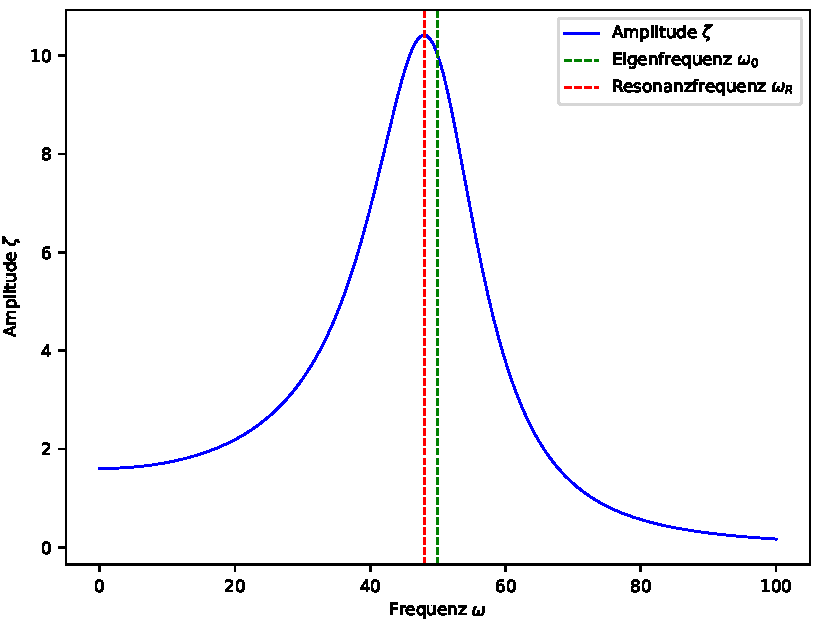
\includegraphics[]{pdf/Lorentzkurve}
        \end{adjustbox}
        \begin{adjustbox}{max width=0.45\linewidth, keepaspectratio}
            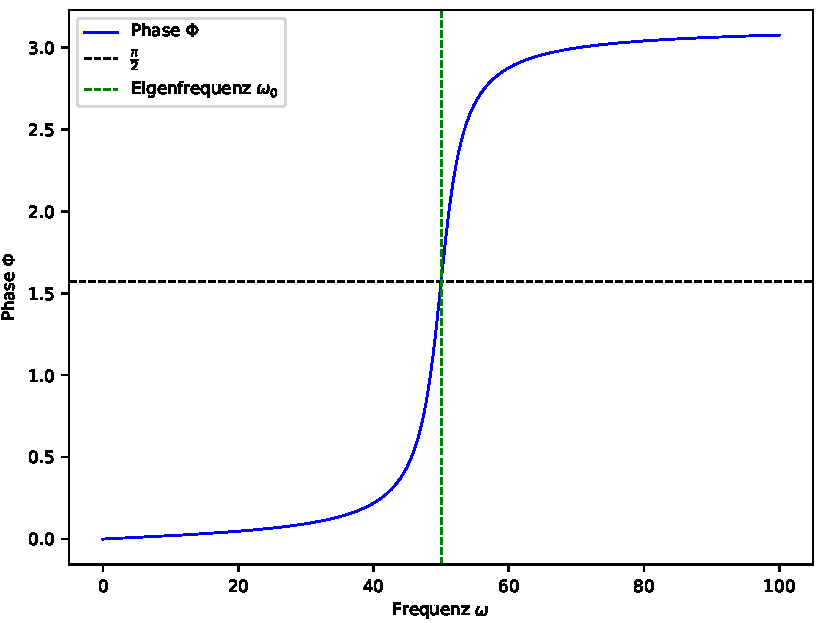
\includegraphics[]{pdf/Phase}
        \end{adjustbox}
        \captionof{figure}{Links: Beispielhafter Verlauf einer Lorentzkurve für $f_0 = 10^7$, $\omega_0 = 50$ und $\gamma = 20$ mit eingezeichneten Werten für Eigenfrequenz $\omega_0$ und Resonanzfrequenz $\omega_R$. Rechts: Beispielhafter Verlauf der Phase für $\omega_0 = 50$ und $\gamma = 5$.}
        \label{fig:Lorentzkurve}
    \end{center}
\endminipage

Im Verlauf der Lorentzkurve erkennt man das charakteristische Resonanzverhalten.
Sie hat ihr Maximum bei der Resonanzfrequenz $\omega_R$:
\begin{align}
    \label{eq:Resonanzfrequenz}
    \omega_R &= \sqrt{\omega_0^2 - \frac{\gamma^2}{2}}.
\end{align}

An der Phase ist zu erkennen, dass die Oszillatorschwingung hinter der Anregung her schwingt, im Resonanzfall genau um $\frac{\pi}{2}$ verzögert.

Die Ausprägung des Peaks der Lorentzkurve ist abhängig von der Dämpfung $\gamma$ des Oszillators.
Je kleiner $\gamma$, desto ausgeprägter ist der Peak.

Als Maß hierfür definieren wir die Güte
\begin{align}
    \label{eq:Guete}
    Q = \frac{\omega_0}{\gamma} = 2 \pi \frac{E}{|\Delta E|}.
\end{align}

Diese gleicht dem Energieverlust pro Schwingung eines theoretischen ungetriebenen Oszillators mit sonst gleichen Eigenschaften.

\subsubsection*{Harmonische Wellen}

Breitet sich eine Schwingung in Raum und Zeit aus, so entsteht eine Welle.
Eine harmonische Welle die sich in $x$-Richtung ausbreitet wird beschrieben durch
\begin{align*}
    \frac{\partial^2 z}{\partial t^2} &= v_\mathrm{ph}^2 \; \frac{\partial^2 z}{\partial x^2}.
\end{align*}

Dabei ist $z$ die Auslenkung und $v_\mathrm{ph}$ die Phasengeschwindigkeit der Welle.

Wenn der Raum in dem sich die Welle ausbreiten kann durch Randbedingungen beschränkt ist ergibt sich eine stehende Welle.
Die Welle wird an einer Berandung reflektiert und die ausfallende Welle überlagert sich mit der einfallenden.

Ist ein eindimensional schwingendes System, etwa bei $x=0$ und $x=l$ fixiert, die Amplitude also immer Null, so gilt für die Wellenlängen der entstehenden Welle:
\begin{align}
    \lambda_n &= \frac{2l}{n}, \hspace{1cm} n=1,2,3,...
\end{align}

Diese stehenden Wellen können als Eigenschwingungen des Systems betrachtet werden.
Deren Frequenzen
\begin{align}
    \nu_n = \frac{v_\mathrm{ph}}{\lambda_n} = \frac{v_\mathrm{ph} n}{2 l}
\end{align}

sind ganzzahlige vielfache der Grundfrequenz $\nu_1$ und werden als Oberschwingungen bezeichnet.

\subsubsection*{Erzwungene gedämpfte Biegeschwingung eines elastischen Reeds}

Im Versuch benutzen wir die elastische Biegeschwingung eines metallenen Reeds.
Die genaue mathematische Herleitung der Differentialgleichung dieses Systems ist sehr umfangreich.
Dafür verweisen wir auf die in der Versuchsanleitung \cite{Anleitung} bereits eingeführte Diplomarbeit \cite{Diplomarbeit} von Johannes Claßen.
Hier geben wir lediglich das Ergebnis und die sich daraus ergebenden Konsequenzen für unser Experiment an.
Die transversale Auslenkung $z$ eines kleinen Teil des Reeds an der Position $x$ wird durch
\begin{align}
    \label{eq:TransversaleAuslenkung}
    \frac{\partial^2 z}{\partial t^2} + \frac{d^2}{12} v_{\Upsilon}^2 \frac{\partial^4 z}{\partial x^4} = f_0 e^{i \omega t} \delta(x-l)
\end{align}

bestimmt.
Dabei sind $d$ und $l$ die Dicke und Länge des Reeds und $v_{\Upsilon} = \sqrt{\frac{E}{\rho}}$ die Schallgeschwindigkeit im Reed.

Auch diese Schwingung zeigt Resonanzverhalten und lässt sich um die Maxima herum durch die Lorentzkurve approximieren.

Die diskreten Eigenfrequenzen liegen bei
\begin{align}
    \label{eq:Eigenfrequenzen}
    \nu_n &= \alpha_n (2n+1)^2 \frac{\pi}{16\sqrt{3}} \frac{d}{l^2} v_{\Upsilon}, \hspace{1cm} n=0,1,2,...
    \intertext{mit den numerischen Konstanten}
    \alpha_0 = 1,424987 \hspace{0.5cm} \alpha_1 &= 0,992249 \hspace{0.5cm} \alpha_2 = 1,000198
\end{align}

Damit ergeben sich feste Frequenzverhältnisse zwischen den verschiedenen Schwingungsmoden
\begin{align}
    \frac{\nu_1}{\nu_0} = 6.267
    \hspace{0.5cm}
    \frac{\nu_2}{\nu_0} = 17.548
    \label{eq:VerhaeltnisseEigenfrequenzen}
\end{align}

\subsection{Messung am experimentellen Aufbau}

Der schematische Aufbau des Experiments ist in Abbildung \ref{fig:SchemaVersuchsaufbau} dargestellt.

\minipage{\linewidth}
    \begin{center}
        \captionsetup{type=figure}
        \begin{adjustbox}{max width=\linewidth, keepaspectratio}
            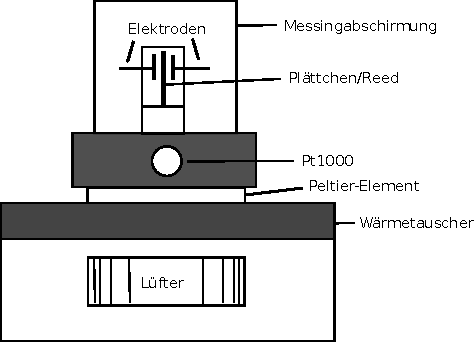
\includegraphics[]{pdf/Versuchsaufbau}
        \end{adjustbox}
        \captionof{figure}{Schematischer Versuchsaufbau (Vorlage Versuchsanleitung \cite{Anleitung})}
        \label{fig:SchemaVersuchsaufbau}
    \end{center}
\endminipage

Um einen wichtigen Aspekt für die spätere Auswertung der Messdaten zu erkennen, ist es nötig, sich die Beziehung der wirkenden Kraft herzuleiten.
Als Grundlage der Herleitung verwenden wir die Kraft zwischen zwei Kondensatorplatten:
\begin{align}
    \label{eq:KraftKondensatorplatten}
    \begin{split}
        F = \frac{C_a U^2}{2 g_a}
    \end{split}
\end{align}

Mithilfe der Kapazität der Anregungselektrode
\begin{align}
    \label{eq:KapazitaetAnregungselektrode}
    \begin{split}
        C_a = \frac{\varepsilon_0 S}{g_a}
    \end{split}
\end{align}

und einer angelegten Wechselspannung $U(t) = U_0 \cos \omega t$ erhalten wir die periodische Kraft, welche unsere Schwingung anregt
\begin{align}
    \label{eq:PeriodischeKraft}
    \begin{split}
        F \left( t \right) = \frac{C_a {U_0}^2}{4 g_a} \left( 1 + \cos 2 \omega t \right).
    \end{split}
\end{align}

Wir erkennen: \textbf{Die Frequenz der Schwingung wird doppelt so groß sein wie die eingestellte Frequenz unseres Erregers.}

Analog lässt sich über die Kapazität der Detektionselektrode
\begin{align}
    \label{eq:KapazitaetDetektionselektrode}
    \begin{split}
        C_d = \frac{\varepsilon_0 S}{g_d}
    \end{split}
\end{align}

eine Beziehung zwischen Schwingung und gemessener Spannung herleiten.
Die Spannung der Detektionselektrode lässt sich schreiben als
\begin{align}
    \label{eq:Detektionselektrode}
    \begin{split}
        U_d &= U_B \frac{z}{g_d} \frac{C_d}{C_d + C_L} \frac{\omega R \left( C_d + C_L \right)}{\sqrt{1+\left( \omega R \left( C_d + C_L \right) \right)^2}}
    \end{split}
\end{align}

wobei wir uns zunächst von der Frequenzunabhängigkeit des Übertragungsverhältnisses $\left| \frac{U_d}{z} \right|$ überzeugen möchten.

Dazu kann für den im Experiment verwendeten Frequenzbereich von $\frac{\omega}{2\pi} > \SI{100}{\hertz}$ der letzte Faktor in Gleichung \ref{eq:Detektionselektrode} (entspricht Gleichung 2.6 der Versuchsanleitung \cite{Anleitung}) in guter Näherung durch \SI{1}{} ersetzt werden.
Der Verlauf des Faktors in Abhängigkeit von $\omega$ ist in Abbildung \ref{fig:Faktor} dargestellt.

\minipage{\linewidth}
    \begin{center}
        \captionsetup{type=figure}
        \begin{adjustbox}{max width=\linewidth, keepaspectratio}
            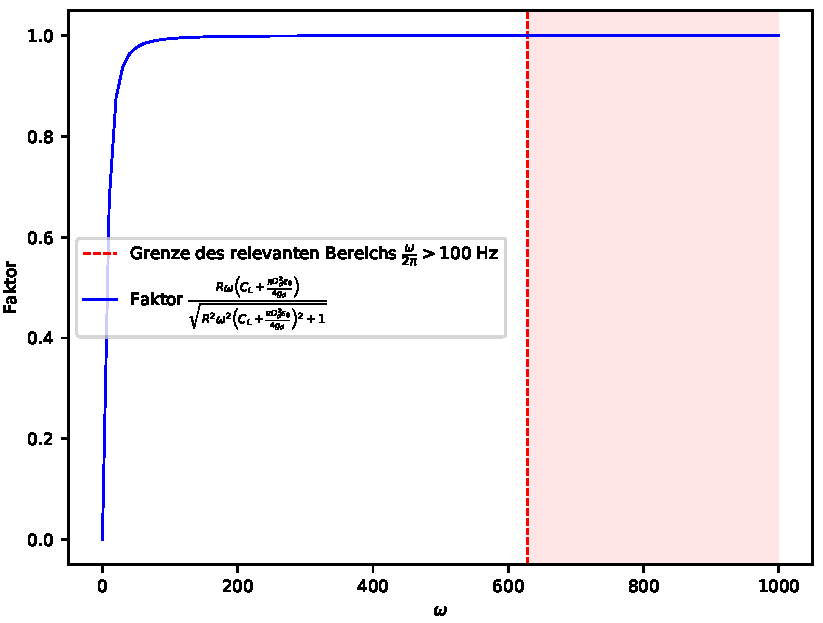
\includegraphics[]{pdf/Faktor}
        \end{adjustbox}
        \captionof{figure}{Letzter Faktor in Gleichung \ref{eq:Detektionselektrode} kann in guter Näherung durch \SI{1}{} ersetzt werden.}
        \label{fig:Faktor}
    \end{center}
\endminipage

Außerdem stellen wir fest, dass $C_d \ll C_L$ und können somit insgesamt schreiben
\begin{align}
    \label{eq:DetektionselektrodeVereinfacht}
    \begin{split}
        U_d &\approx U_B \frac{z}{g_d} \frac{C_d}{C_L}
    \end{split}
\end{align}

Diese Beziehung lässt sich also dazu verwenden, zu den im Experiment gemessenen Werten für $U_d$ die entsprechende Auslenkung $z$ der Schwingung zu berechnen.

\subsection{Einige Abschätzungen zur Vorbereitung}

Um uns die Dimensionen des Experiments deutlich zu machen, berechnen wir nun den erwarteten Maximalwert des Amplitudenverlaufs $\zeta$.
Wir nutzen Gleichung 2.8 der Versuchsanleitung
\begin{align}
    \label{eq:MaximaleAmplitude}
    \begin{split}
        \zeta_0 = 4 \frac{l^3}{Ed^3b} F_0
    \end{split}
\end{align}

wobei $F_0$ der Maximalwert der periodischen Anregungskraft nach Gleichung \ref{eq:PeriodischeKraft} ist.

Damit lässt sich nun auch der Maximalwert der Spannung der Detektionselektrode $U_d$ nach Gleichung \ref{eq:DetektionselektrodeVereinfacht} bestimmen.
Wir erhalten die beiden Werte $\zeta_0 = \SI{2.55}{\nano\meter}$ und $U_{d0} = \SI{5.76}{\micro\volt}$.

\textbf{Die abgeschätzten Größenordnung unserer Messgrößen bestätigen also die Notwendigkeit eines Verstärkers.}

\subsection{Theoretische Werte für die erwarteten Eigenfrequenzen}

Mithilfe Gleichung \ref{eq:Eigenfrequenzen} und den Angaben zum Reed in der Versuchsanleitung \cite{Anleitung} lassen sich die erwarteten Eigenfrequenzen abschätzen.
Das erleichtert uns während des Experiments die Suche nach den tatsächlichen Resonanzkurven.

Wir erhalten $\nu_{0 theo} = \SI{274}{\hertz}$, $\nu_{1 theo} = \SI{1719}{\hertz}$ und $\nu_{2 theo} = \SI{4812}{\hertz}$.
\label{eq:AbschaetzungEigenfrequenzen}

\subsection{Statistische Grundlagen}

Eine Einführung in die statistischen Grundlagen, die wir beispielsweise als Basis zur Erstellung der Fits an die Messdaten verwendet haben, würde den Umfang dieses Texts sprengen.
Wir verweisen daher an dieser Stelle auf die entsprechenden Kapitel der Versuchsanleitung \cite{Anleitung}.

\section{Durchführung}

\subsubsection*{Aufbau}

\colorbox{yellow}{TODO Skizze oder Schema von Versuchsaufbau}

\colorbox{yellow}{TODO Aufbau in Worten erklären und Schema-Grafik referenzieren}

\subsubsection*{Einstellungen}

Anschließend überprüfen wir die Einstellungen am Lock-In Verstärker.
Dabei nutzen wir hauptsächlich die vorgegebenen Werte aus der Versuchsanleitung \cite{Anleitung} sowie einzelne Modifikationen unter der Anleitung des Assistenten.
Die endgültigen Einstellungen sind in Tabelle \ref{tab:EinstellungenVerstaerker} aufgetragen.

\minipage{\linewidth}
    \begin{center}
        \captionsetup{type=table}
        \begin{adjustbox}{max width=\linewidth, keepaspectratio}
            \begin{tabular}{lllll}
            \toprule
            Vorderseite    & ~        & ~                       & Rückseite      & ~                \\
            \midrule
            SIGNAL FILTERS & BANDPASS & IN                      & SINE AMPLITUDE & \SI{1}{\volt}    \\
            ~              & LINE     & IN                      & VCO RANGE      & \SI{100}{\hertz} \\
            ~              & LINEx2   & IN                      & ~              & ~                \\
            SENSITIVITY    & ~        & \SI{100}{\micro\volt}   & ~              & ~                \\
            DYN RES        & ~        & LOW                     & ~              & ~                \\
            TIME CONSTANT  & PRE      & \SI{300}{\milli\second} & ~              & ~                \\
                           & POST     & \SI{0.1}{\second}       & ~              & ~                \\
            REFERENCE      & PHASE    & -90 DEG                 & ~              & ~                \\
            ~              & MODE     & 2f                      & ~              & ~                \\
            ~              & TRIG     & $\sim$                  & ~              & ~                \\
            CHANNEL 1/2    & OFFSET   & OFF                     & ~              & ~                \\
            ~              & EXPAND   & X1                      & ~              & ~                \\
            \bottomrule
            \end{tabular}
        \end{adjustbox}
        \captionof{table}{Einstellungen am Lock-In Verstärker}
        \label{tab:EinstellungenVerstaerker}
    \end{center}
\endminipage

\subsubsection*{LabVIEW}

Der Tutor gibt zu Beginn des Versuchs eine kurze, hilfreiche Einweisung zu LabVIEW.
Zudem stehen uns mehrere LabVIEW-Beispielskripte auf der Versuchs-Homepage zur Verfügung.

\colorbox{yellow}{TODO Schritt für Schritt erklären, wie unser Skript entsteht}

\subsubsection*{Heizspannung des Peltier-Elements}

Parallel zur Entwicklung unseres LabVIEW-Skripts für die eigentliche Messung, ändern wir die Heizspannung des Peltier-Elements.
Dabei erhöhen wir die Spannung immer wieder um \SI{0.1}{\volt} und warten anschließend bis sich eine neue Gleichgewichts-Temperatur eingependelt hat.
Die Temperatur bestimmen wir in regelmäßigen Abständen manuell per Gleichung 3.1 der Versuchsanleitung \cite{Anleitung}.
Als Grenze sollen \SI{60}{\celsius} nicht überschritten werden.

Wir können so für die spätere komplette Messung den Bereich der Heizspannung des Peltier-Elements auf \SIrange{0}{0.9}{\volt} bestimmen.

Nachdem die Bestimmung des Bereichs der Heizspannung abgeschlossen ist, wird die Betriebsspannung des Peltier-Element wieder auf \SI{0}{\volt} gesetzt.

\subsubsection*{Resonanzfrequenz der ersten Mode als Anhaltspunkt}

Wir wollen in einer ersten Messung die Resonanzfrequenz der ersten Mode bestimmen.
Diese sollte im Vergleich zu den höheren Moden den Vorteil haben, dass sie eine größere Amplite besitzt.
\colorbox{yellow}{TODO Begründung?}
Wir erhoffen uns davon, dass sie besser auffindbar ist.

Grundsätzlich tragen sowohl eine große Anzahl an Messpunkten, als auch ein großer Messbereich zu einer langen Messdauer bei.
Um die Dauer der Messung in einem akzeptablen Rahmen zu halten, ist es daher sinnvoll die vorher gemachten Abschätzungen aus der Einleitung zu verwenden.
Wir wissen so, in welchem Bereich die Resonanzfrequenz der ersten Mode etwa zu erwarten ist.
\colorbox{yellow}{TODO Referenz zur Abschätzung in der Einleitung einfügen}

Leider lassen sich unsere zunächst aufgenommenen Daten einer detaillierteren Messung rund um den erwarteten Bereich für die Resonanzfrequenz der ersten Mode nicht verwenden.
Es stellt sich heraus, dass statt der erwarteten Resonanzkurve eine Oberschwingung der \SI{50}{\hertz} Netzfrequenz des Stromnetzes vermessen wurde.
\colorbox{yellow}{TODO Haben wir die Daten dazu nicht gespeichert?}
Der Messbereich muss also für eine erfolreiche Suche nach der Resonanzfrequenz der ersten Mode noch deutlich erweitert werden.

\subsubsection*{Abschließende Messung}

Mit den aktualisierten Suchbereich lässt sich ein weiterer Peak auffinden.
Er gehört zu einer Kurve von Messpunkten mit dem charakteristischem Verlauf einer Resonanzkurve.
Mit diesem ersten Wert für die Resonanzfrequenz der ersten Mode lassen sich mithilfe von Gleichung 1.24 der Versuchsanleitung \cite{Anleitung} die Frequenzen für höhere Moden bestimmen.
Wir definieren schließlich die drei Messbereiche für die Messung der Resonanzkurven der ersten drei Moden und starten die abschließende Messung, welche die endgültigen Messdaten für unsere Auswertung liefert.

\section{Auswertung}
%
\subsubsection*{Verstärkerschaltung mit einem Transistor in Emitterschaltung}
%
Um einen Vergleich von $I_{\text{C}}$ während des Experiments mit dem zuvor berechneten, theoretischen Wert anzustellen, muss $I_{\text{C}}$ über die mit dem Multimeter bestimmte $U_{\text{C}}$ bestimmt werden:
%
\begin{align}
    \label{eq:ICausUC}
    \begin{split}
        I_C &= \frac{U_C}{R_C}
    \end{split}
    \\
    \label{eq:FehlerICausUC}
    \begin{split}
        \Delta I_C &= \sqrt{ \left ( \frac{1}{R_C} \cdot \Delta U_C \right ) ^2 + \left ( - \frac{U_C}{{R_C}^2} \cdot \Delta U_C \right ) ^2 }
    \end{split}
\end{align}
%
Die Verstärkung $V_U$ berechnet sich aus dem Quotienten von $U_{\text{SS}}$ des Ausgangssignals zu $U_{\text{SS}}$ des Eingangssignals.
Der Frequenzgang wird geplottet und ist in Abbildung \ref{fig:FrequenzgangEmitterschaltung} dargestellt.
Die untere Grenzfrequenz wird über eine Horizontale beim $\nicefrac{1}{\sqrt{2}}$-fachen des Plateaus ermittelt.
Die Vergleiche zwischen den experimentell bestimmten Werten und den Theoriewerten sind in Tabelle \ref{tab:VergleichExpTheo} aufgeführt.
%
\par
%
Auf eine detailliertere Angabe von Formeln zur Berechnung der einzelnen Größen und Messunsicherheiten wird an dieser Stelle verzichtet.
%
\par
%
\minipage{\linewidth}
    \begin{center}
        \captionsetup{type=figure}
        \begin{adjustbox}{max width=\linewidth, keepaspectratio}
            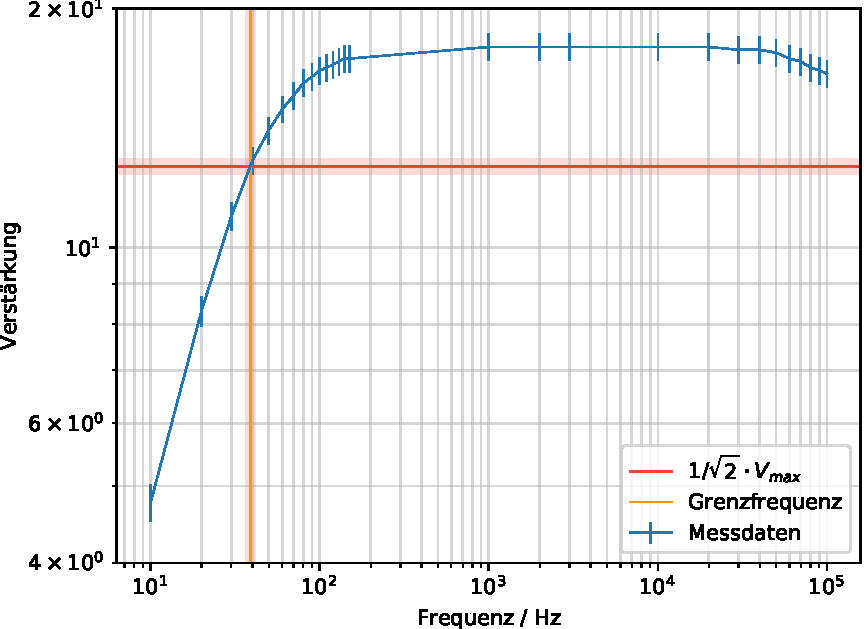
\includegraphics[]{pdf/FrequenzgangEmitterschaltung}
        \end{adjustbox}
        \captionof{figure}{Frequenzgang der Emitterschaltung}
        \label{fig:FrequenzgangEmitterschaltung}
    \end{center}
\endminipage
%
\subsubsection*{Verstärkerschaltung mit einem Transistor in Kollektorschaltung}
%
Falls im Folgenden nicht weiter beschrieben, finden die Berechnungen analog der Auswertung zum vorherigen Versuchsteil statt.
Für die Berechnung der Kabellänge wird eine Ausbreitungsgeschwindigkeit von $v = \nicefrac{2}{3} \cdot c$ angenommen, wobei $c$ die Lichtgeschwindigkeit beschreibt mit $c = \SI{299800}{\kilo\meter\per\second}$ \cite{Anleitung}.
Die Länge $L$ des Kabels berechnet sich mit:
%
\begin{align}
    \label{eq:Kabellaenge}
    \begin{split}
        L &= v \cdot t
    \end{split}
    \\
    \label{eq:FehlerKabellaenge}
    \begin{split}
        \Delta L &= v \cdot \Delta t
    \end{split}
\end{align}
%
Der Frequenzgang ist in Abbildung \ref{fig:FrequenzgangKollektorschaltung} dargestellt.
Die Vergleiche zwischen den experimentell bestimmten Werten und den Theoriewerten sind in Tabelle \ref{tab:VergleichExpTheo} aufgeführt.
%
\par
%
\minipage{\linewidth}
    \begin{center}
        \captionsetup{type=figure}
        \begin{adjustbox}{max width=\linewidth, keepaspectratio}
            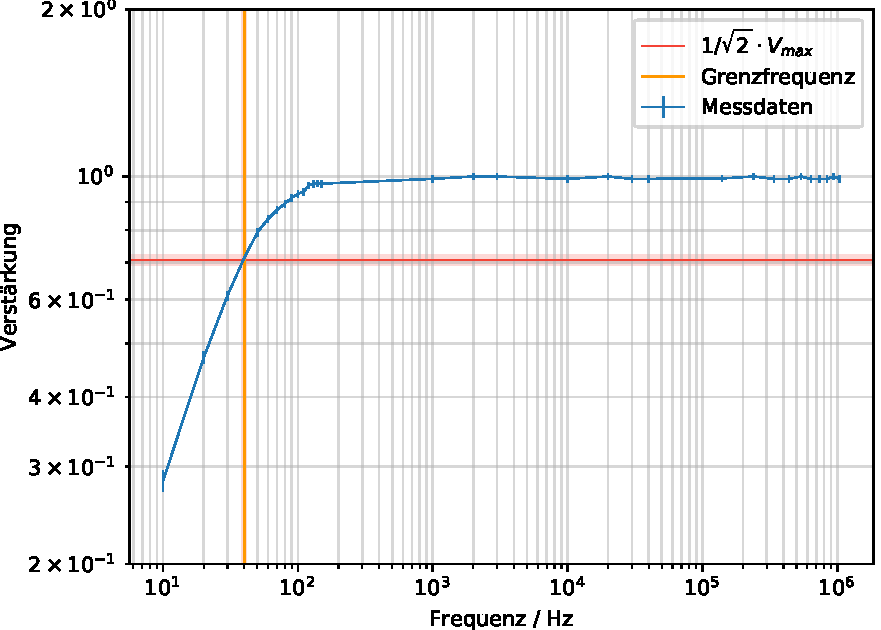
\includegraphics[]{pdf/FrequenzgangKollektorschaltung}
        \end{adjustbox}
        \captionof{figure}{Frequenzgang der Kollektorschaltung}
        \label{fig:FrequenzgangKollektorschaltung}
    \end{center}
\endminipage
%
\subsubsection*{Vergleichstabelle}
%
\minipage{\linewidth}
    \begin{center}
        \captionsetup{type=table}
        \begin{adjustbox}{max width=\linewidth, keepaspectratio}
            \begin{tabular}{lllll}
            \toprule
            Versuchsteil       & Größe             & Experimentell & Theoriewert & Abweichung \\
            \midrule
            Emitterschaltung   & $U_{\text{CE}}$   & \SI{7,85 \pm 0,05}{\volt}           & \SI{7,87 \pm 0,07}{\volt}        & \SI{0,24}{\sigma} \\
            ~                  & $U_{\text{BE}}$   & \SI{0,628 \pm 0,005}{\volt}         & \SI{0,66 \pm 0,08}{\volt}        & \SI{0,4}{\sigma}  \\
            ~                  & $U_{\text{C}}$    & \SI{6,82 \pm 0,05}{\volt}           & \SI{6,80 \pm 0,07}{\volt}        & \SI{0,23}{\sigma} \\
            ~                  & $U_{R_1}$         & \SI{14,03 \pm 0,05}{\volt}          & \SI{14,01 \pm 0,08}{\volt}       & \SI{0,21}{\sigma} \\
            ~                  & $U_{R_2}$         & \SI{0,958 \pm 0,005}{\volt}         & \SI{0,99 \pm 0,08}{\volt}        & \SI{0,4}{\sigma}  \\
            ~                  & $I_{\text{C}}$    & \SI{0,958 \pm 0,005}{\milli\ampere} & \SI{1}{\milli\ampere}            & \SI{0,25}{\sigma} \\
            ~                  & $V_U$             & \SI{17,9 \pm 0,7}{}                 & \SI{20,61 \pm 0,29}{}            & \SI{2,7}{\sigma}  \\
            ~                  & $f_{\text{uG}}$   & \SI{39 \pm 2}{\hertz}               & \SI{36 \pm 6}{\hertz}            & \SI{0,5}{\sigma}  \\
            ~                  & $R_{\text{Ein}}$  & \SI{45,4 \pm 1,0}{\kilo\ohm}        & \SI{44 \pm 6}{\kilo\ohm}         & \SI{0,16}{\sigma} \\
            ~                  & $R_{\text{Aus}}$  & \SI{5,8 \pm 1,0}{\kilo\ohm}         & \SI{6,80 \pm 0,07}{\kilo\ohm}    & \SI{1}{\sigma}    \\
            Kollektorschaltung & $U_{\text{E}}$    & \SI{7,56 \pm 0,05}{\volt}           & \SI{7,52 \pm 0,08}{\volt}        & \SI{0,4}{\sigma}  \\
            ~                  & $U_{\text{BE}}$   & \SI{0,660 \pm 0,005}{\volt}         & \SI{0,66 \pm 0,08}{\volt}        & \SI{0,01}{\sigma} \\
            ~                  & $U_{R_1}$         & \SI{6,70 \pm 0,05}{\volt}           & \SI{6,82 \pm 0,11}{\volt}        & \SI{1,0}{\sigma}  \\
            ~                  & $U_{R_2}$         & \SI{8,25 \pm 0,05}{\volt}           & \SI{8,18 \pm 0,11}{\volt}        & \SI{0,6}{\sigma}  \\
            ~                  & $I_{\text{E}}$    & \SI{16,09 \pm 0,19}{\milli\ampere}  & \SI{15,9 \pm 0,1}{\milli\ampere} & \SI{1,1}{\sigma}  \\
            ~                  & $V_U$             & \SI{0,99 \pm 0,03}{}                & \SI{0,92 \pm 0,04}{}             & \SI{1,1}{\sigma}  \\
            ~                  & $f_{\text{uG}}$   & \SI{40 \pm 1}{\hertz}               & \SI{41 \pm 5}{\hertz}            & \SI{0,2}{\sigma}  \\
            ~                  & Kabellänge $L$    & \SI{20,0 \pm 0,4}{\meter}           & \SI{20}{\meter}                  & \SI{0,07}{\sigma} \\
            ~                  & Kabelimpedanz $R$ & \SI{70 \pm 20}{\ohm}                & \SI{50}{\ohm}                    & \SI{1}{\sigma}    \\
            \bottomrule
            \end{tabular}
        \end{adjustbox}
        \captionof{table}{Vergleich der experimentell bestimmten Werte mit den Theoriewerten}
        \label{tab:VergleichExpTheo}
    \end{center}
\endminipage

\section{Kritische Würdigung}

\subsubsection*{Vergleich der bestimmten Eigen- respektive Resonanzfrequenzen}

\colorbox{yellow}{TODO}

\subsubsection*{Interpretation der Abschätzung systematischer Fehler}

\colorbox{yellow}{TODO}

\subsubsection*{Vergleich der bestimmten Werte für die Güte}

\colorbox{yellow}{TODO}

\subsubsection*{Temperaturabhängigkeit der Resonanzfrequenzen}

\colorbox{yellow}{TODO}

\subsubsection*{Analyse möglicher Fehlerquellen}

\colorbox{yellow}{TODO}

\subsubsection*{PyVISA als Alternative zu LabVIEW}

\colorbox{yellow}{TODO}

\subsubsection*{Simulation des kompletten Versuchs}

\colorbox{yellow}{TODO}

\section{Quellenangaben}

\printbibliography[heading=none]

\newpage
\section{Anhang}

\minipage{\linewidth}
    \begin{center}
        \captionsetup{type=figure}
        \begin{adjustbox}{max height=0.5\textheight, keepaspectratio}
            \includegraphics[angle=90, origin=c]{png/LabVIEW}
        \end{adjustbox}
        \captionof{figure}{Screenshot des für die Messung verwendeten LabVIEW-Skripts (um \SI{90}{\degree} gedreht)}
        \label{fig:LabVIEWSkript}
    \end{center}
\endminipage


\end{document}
